%----------------------------------------------------------------------------------------
%	PACKAGES AND THEMES
%----------------------------------------------------------------------------------------
\PassOptionsToPackage{table}{xcolor}
\documentclass[aspectratio=169,xcolor=dvipsnames,svgnames,x11names,fleqn]{beamer}
% \documentclass[aspectratio=169,xcolor=dvipsnames,fleqn]{beamer}

\usetheme{RedVelvet}

\usefonttheme[onlymath]{serif}



\usepackage{xspace}
\usepackage{amsmath}
\usepackage{amssymb}
\usepackage{amsfonts}
\usepackage{color}
\usepackage{physics}
% \usepackage{mathbb}
\usepackage{rahul_math}
\usepackage{bigints}
\usepackage{hyperref}

\usepackage{graphicx} % Allows including images
\usepackage{booktabs} % Allows the use of \toprule, \midrule and \bottomrule in tables
\usepackage{tikz,pgfplots}
\usepackage{subfigure}
\usetikzlibrary{arrows}
\usepackage{minted}
\definecolor{LightGray}{gray}{0.9}
\definecolor{cream}{rgb}{0.92, 0.9, 0.55}
\definecolor{lightblue}{rgb}{0.68, 0.85, 0.9}


\usepackage{xcolor-material}
\usetikzlibrary{fit}
\tikzset{%
apple/.pic={
  \fill [MaterialBrown] (-1/8,0)  arc (180:120:1 and 3/2) coordinate [pos=3/5] (@)-- ++(1/6,-1/7)  arc (120:180:5/4 and 3/2) -- cycle;
  \fill [MaterialLightGreen500] (0,-9/10)  .. controls ++(180:1/8) and ++(  0:1/4) .. (-1/3,  -1) .. controls ++(180:1/3) and ++(270:1/2) .. (  -1,   0) .. controls ++( 90:1/3) and ++(180:1/3) .. (-1/2, 3/4) .. controls ++(  0:1/8) and ++(135:1/8) .. (   0, 4/7)
}
}

\newcommand{\leftdoublequote}{\textcolor{blue}{\scalebox{3}{``}}}

\newcommand{\rightdoublequote}{\textcolor{blue}{\scalebox{3}{''}}}


\usepackage{textcomp}

\usepackage{overpic}

%----------------------------------------------------------------------------------------
%	TITLE PAGE
%----------------------------------------------------------------------------------------

\usepackage{tikz-qtree,tikz-qtree-compat}
\usetikzlibrary{calc}


\title[CPE 486/586: Machine Learning]{CPE 486/586: Machine Learning for Engineers} % The short title appears at the bottom of every slide, the full title is only on the title page
\subtitle{01 Tools for Machine Learning}

\author[Rahul Bhadani] {{\Large \textbf{Rahul Bhadani}}}

\institute[UAH] % Your institution as it will appear on the bottom of every slide, maybe shorthand to save space
{
    Electrical \& Computer Engineering,  The University of Alabama in Huntsville
}
\date

% \titlegraphic{
%    \includegraphics[width=0.4\linewidth]{figures/UAH_primary.png}
% }

\begin{document}

%-------------------------------------------------
\begin{frame}
  \titlepage
\end{frame}

%-------------------------------------------------
\begin{frame}{Outline}
   \tableofcontents
\end{frame}



\section{Command Line Tools and Linux}

\begin{frame}
    \sectionpage
\end{frame}

\begin{frame}{Why Command Line Tools and Linux}

\begin{enumerate}
    \item Download data from another location, webpage or server \begin{center}
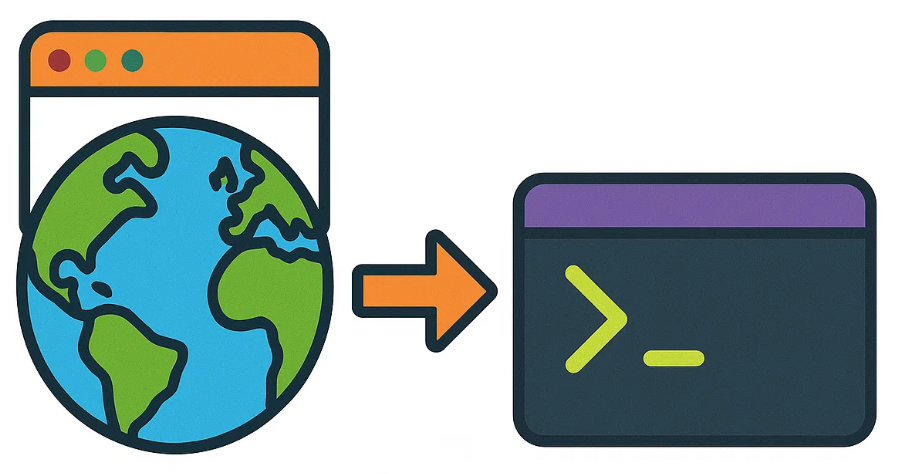
\includegraphics[height=.4\textheight]{Lectures/figures/cmd_line_download.png}
\end{center}
\end{enumerate}
    
\end{frame}

\begin{frame}{Why Command Line Tools and Linux}

\begin{enumerate}
    \item File operation, renaming, copying, editing, etc, in bulk. \begin{center}
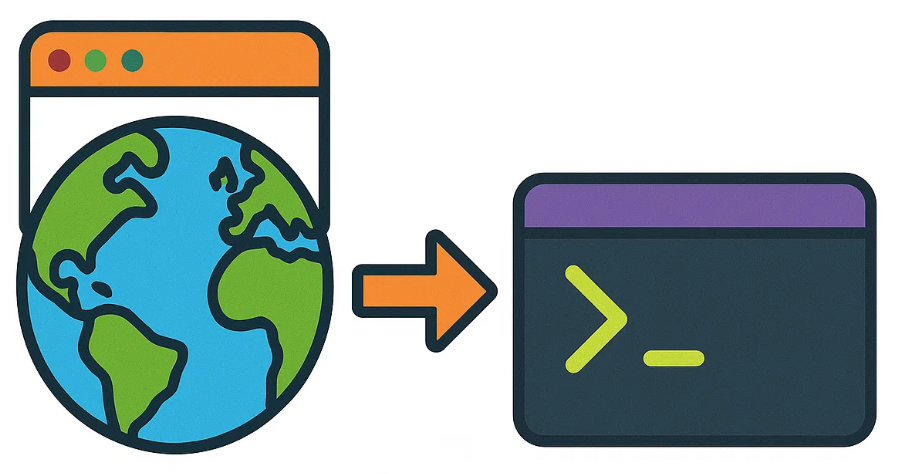
\includegraphics[height=.4\textheight]{Lectures/figures/cmd_line_download.png}
\end{center}
\end{enumerate}
    
\end{frame}

\section{Python}

\begin{frame}
    \sectionpage
\end{frame}

\section{Git and GitHub}

\begin{frame}
    \sectionpage
\end{frame}

\section{Development Environment}

\begin{frame}
    \sectionpage
\end{frame}


\section{Packages and Package Manager}

\begin{frame}
    \sectionpage
\end{frame}


\section{Jupyter Notebook}

\begin{frame}
    \sectionpage
\end{frame}


\section{Markdown}

\begin{frame}
    \sectionpage
\end{frame}

\section{Latex}

\begin{frame}
    \sectionpage
\end{frame}

\section{Other Notable Tools}

\begin{frame}
    \sectionpage
\end{frame}

\begin{frame}
    \Huge{\centerline{\color{bubblegumPink}\textbf{The End}}}
\end{frame}



\end{document}